\documentclass[a4paper, 12pt]{article}
\usepackage[UTF8]{ctex}
\usepackage{float}
\usepackage{graphicx}

\begin{document}
	\title{系统开发工具基础实验报告(二)}
	\author{22110032031 张希敏}
	\date{\today}
	\maketitle
	
	\pagenumbering{roman}
	\tableofcontents
	\newpage
	\pagenumbering{arabic}
	
	\section{练习主题}
	\paragraph{(1)Shell 工具和脚本}
	
	\paragraph{(2)编辑器(Vim)}
	
	\paragraph{(3)数据整理}
	
	\section{练习内容}
	
	\subsection{四个题目}
	
	\subsubsection{题目一}
	阅读 man ls ,然后使用 ls 命令进行如下操作:
	
	(1)输出所有文件(包括隐藏文件)。
	
	(2)文件打印以人类可以理解的格式输出 (例如,使用 454M 而不是 454279954)。
	
	(3)文件以最近访问顺序排序。
	
	(4)以彩色文本显示输出结果。
	
	\paragraph{答:}
	阅读ls的手册,加后缀如下:
	
	(1)所有文件(包括隐藏文件):-a
	
	(2)文件打印以人类可以理解的格式输出: -h
	
	(3)文件以最近访问顺序排序:-t
	
	(4)以彩色文本显示输出结果:--color=auto
	
	\begin{figure}[H]
		\centering
		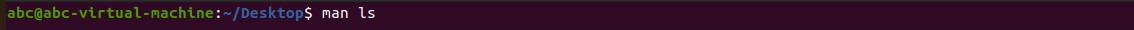
\includegraphics[width=1\textwidth]{002.jpg}
		
\includegraphics[width=1\textwidth]{003.jpg}
		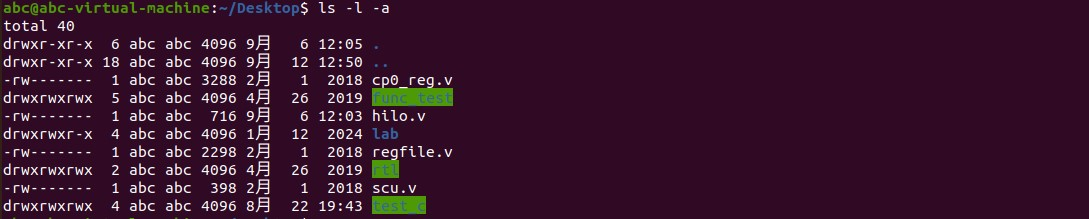
\includegraphics[width=1\textwidth]{004.jpg}
		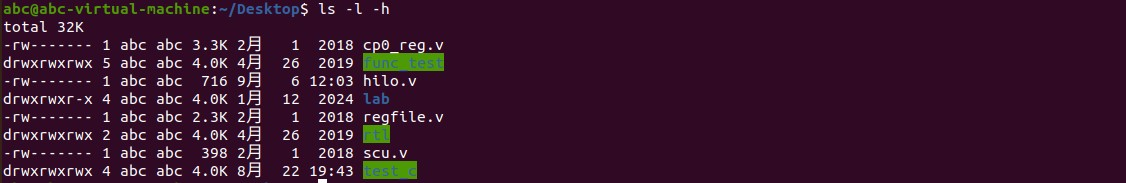
\includegraphics[width=1\textwidth]{005.jpg}
		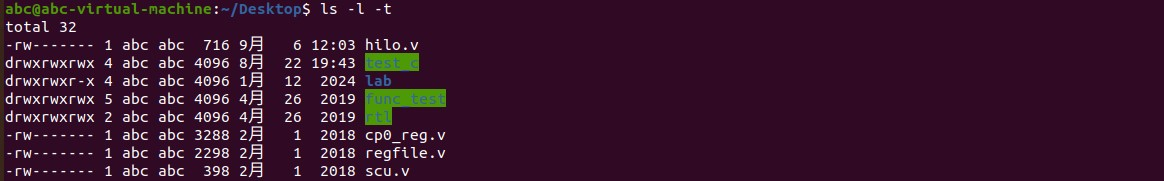
\includegraphics[width=1\textwidth]{006.jpg}
		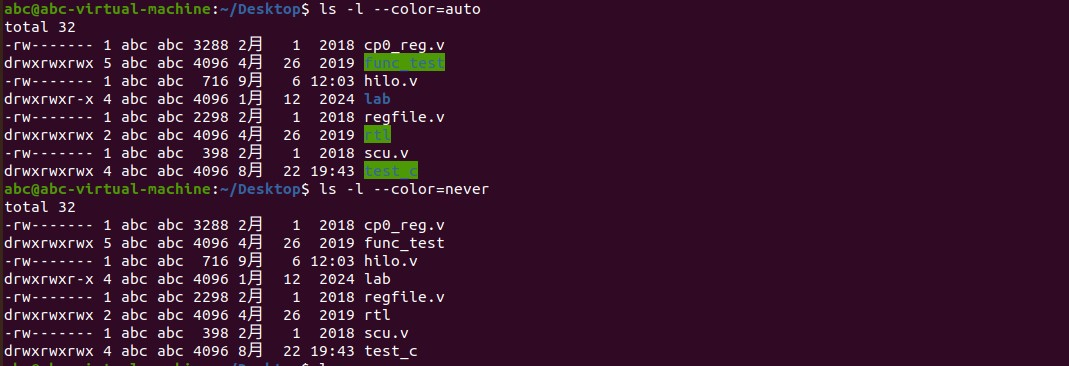
\includegraphics[width=1\textwidth]{007.jpg}
	\end{figure}
	

	\subsubsection{题目二}
	编写两个 bash 函数 marco 和 polo 执行下面的操作。 每当你执行 marco 时,当前的工作目录应当以某种形式保存,当执行 polo 时,无论现在处在什么目录下,都应当 cd 回到当时执行 marco 的目录。 为了方便 debug,你可以把代码写在单独的文件 marco.sh 中,并通过 source marco.sh 命令,(重新)加载函数。
	
	\paragraph{答:}
	如图。代码文件已上传至github。
	
	\begin{figure}[H]
		\centering
		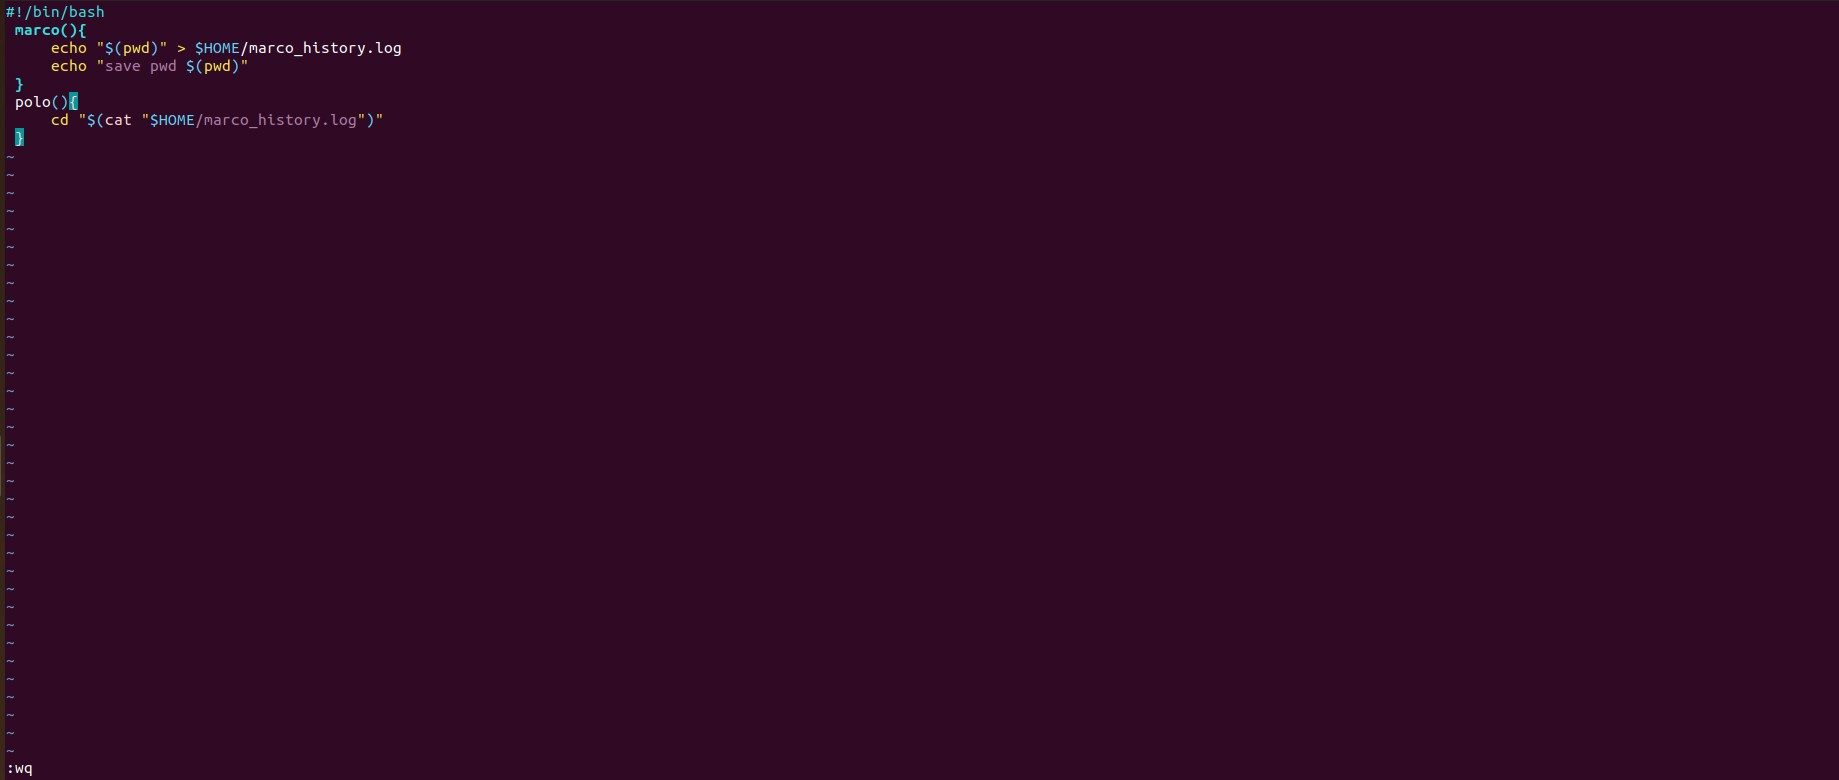
\includegraphics[width=1\textwidth]{008.jpg}
		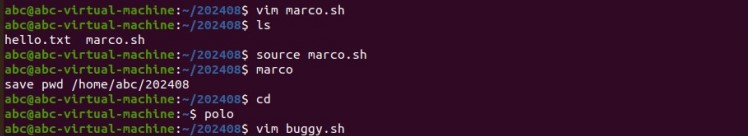
\includegraphics[width=1\textwidth]{009.jpg}
	\end{figure}
	
	\subsubsection{题目三}
	假设您有一个命令,它很少出错。因此为了在出错时能够对其进行调试,需要花费大量的时间重现错误并捕获输出。 编写一段 bash 脚本,运行如下的脚本直到它出错,将它的标准输出和标准错误流记录到文件,并在最后输出所有内容。 加分项:报告脚本在失败前共运行了多少次。
	
	\paragraph{答:}
	如图。代码文件已上传至github。
	
	\begin{figure}[H]
		\centering
		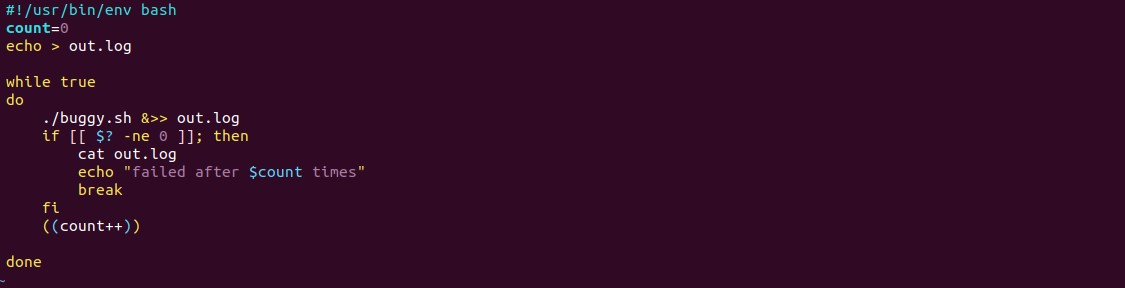
\includegraphics[width=1\textwidth]{010.jpg}
		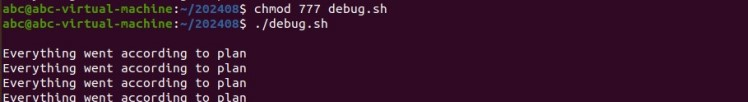
\includegraphics[width=1\textwidth]{011.jpg}
		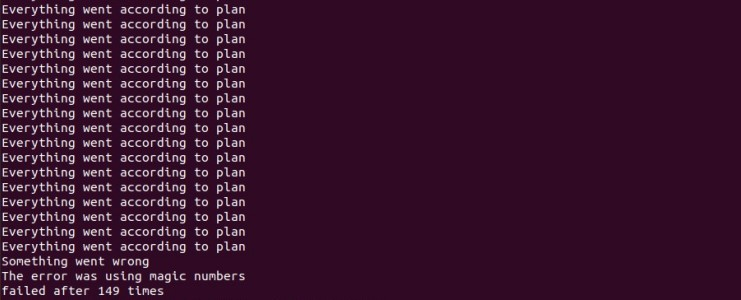
\includegraphics[width=1\textwidth]{012.jpg}
	\end{figure}
	
	\subsubsection{题目四}
	本节课我们讲解的 find 命令中的 -exec 参数非常强大,它可以对我们查找的文件进行操作。但是,如果我们要对所有文件进行操作呢?例如创建一个 zip 压缩文件?我们已经知道,命令行可以从参数或标准输入接受输入。在用管道连接命令时,我们将标准输出和标准输入连接起来,但是有些命令,例如 tar 则需要从参数接受输入。这里我们可以使用 xargs 命令,它可以使用标准输入中的内容作为参数。 例如 ls | xargs rm 会删除当前目录中的所有文件。
	
	你的任务是编写一个命令,它可以递归地查找文件夹中所有的 HTML 文件,并将它们压缩成 zip 文件。注意,即使文件名中包含空格,您的命令也应该能够正确执行。
	
	\paragraph{答:}
	首先使用mkdir命令和touch命令创建文件夹和文件。
	
	\begin{figure}[H]
		\centering
		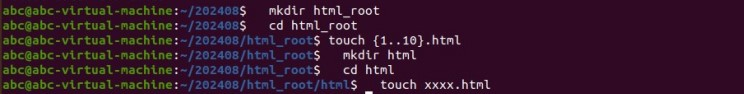
\includegraphics[width=1\textwidth]{015.jpg}
	\end{figure}
	
	然后执行find命令,输入find . -type f -name "*.html" | xargs -d '\\n'  tar -cvzf html.zip
	
	\begin{figure}[H]
	\centering
	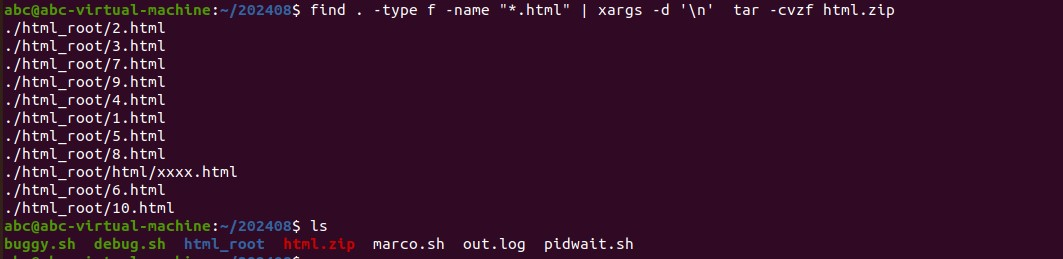
\includegraphics[width=1\textwidth]{016.jpg}
	\end{figure}
	
	\subsection{20个实例}
	
	\paragraph{(1)shell:}
	编写一个命令或脚本递归的查找文件夹中最近使用的文件。更通用的做法,你可以按照最近的使用时间列出文件吗?
	
	\paragraph{答:}
	find . -type f -print0 | xargs -0 ls -lt | head -1
	
	当文件数量较多时,上面的解答会得出错误结果,解决办法是增加 -mmin 条件,先将最近修改的文件进行初步筛选再交给ls进行排序显示:
	
	 find . -type f -mmin -60 -print0 | xargs -0 ls -lt | head -10
	
	\begin{figure}[H]
		\centering
		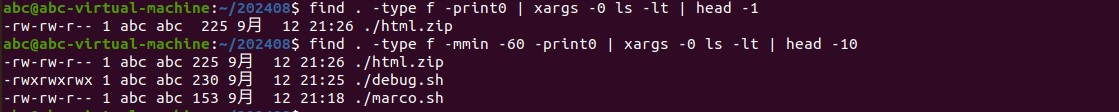
\includegraphics[width=1\textwidth]{017.jpg}
	\end{figure}
	
	\paragraph{(2)vim:}
	用vim编辑器创建一个文件。
	
	\begin{figure}[H]
		\centering
		
\includegraphics[width=1\textwidth]{018.jpg}
		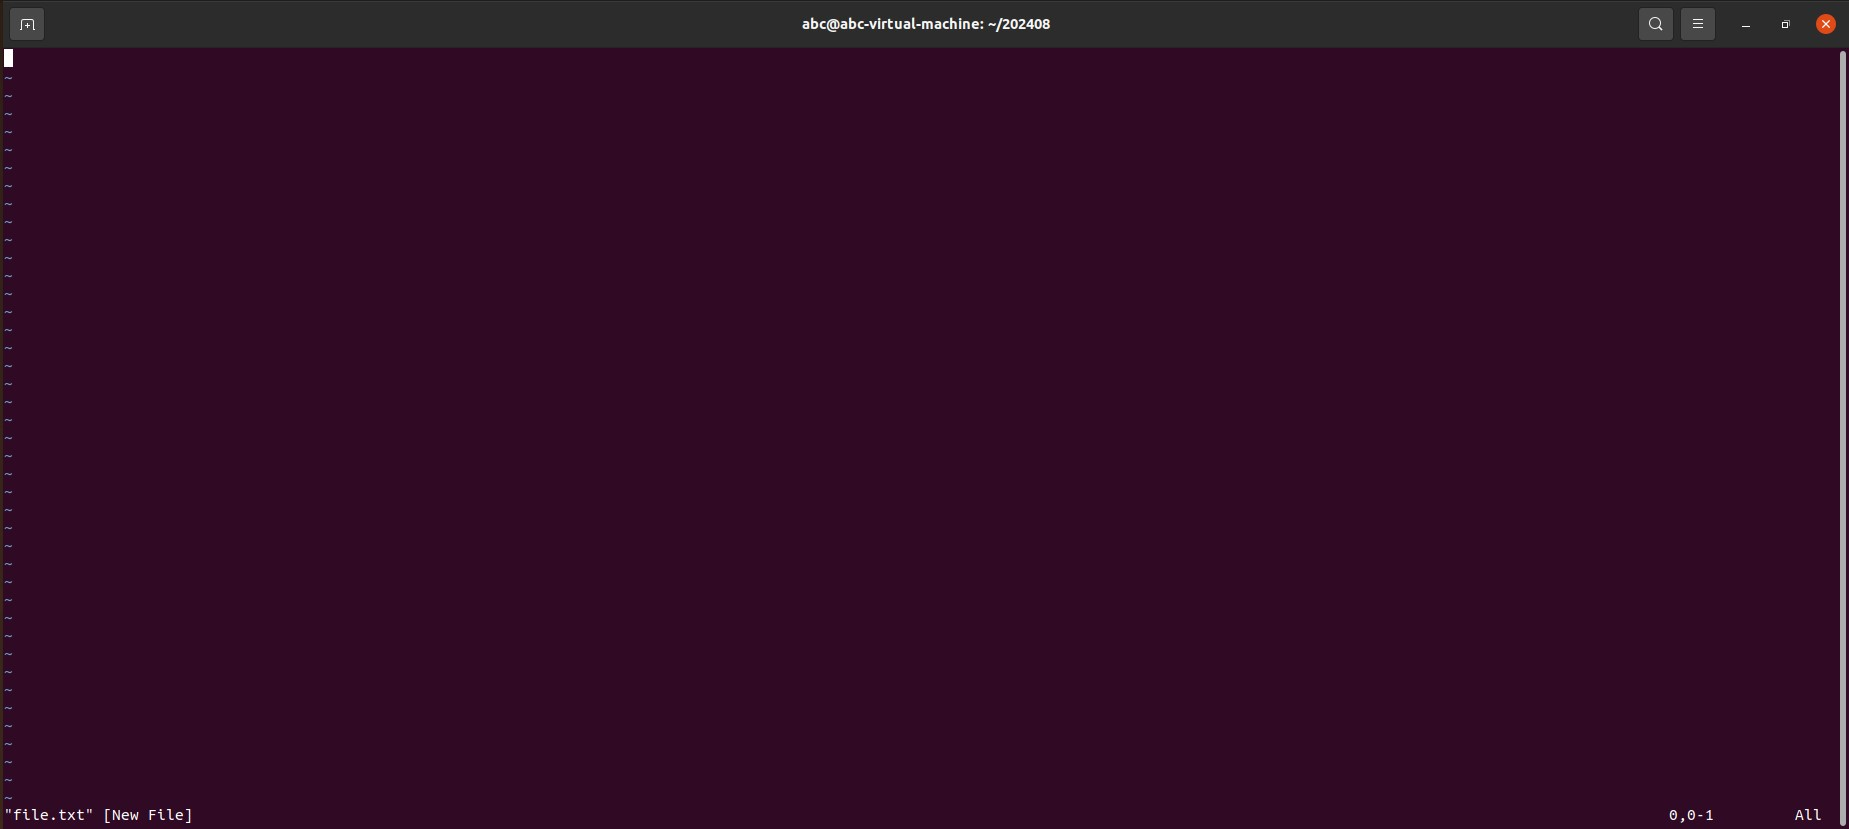
\includegraphics[width=1\textwidth]{019.jpg}
	\end{figure}
	
	\paragraph{(3)vim:}	
	按下i键切换输入模式,在文件中输入一段文字。
	
	\begin{figure}[H]
		\centering
		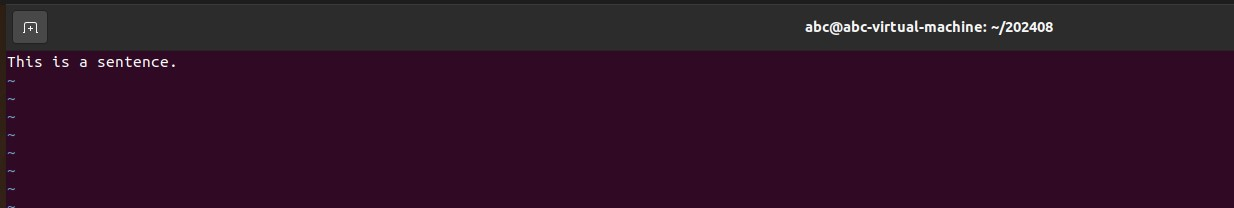
\includegraphics[width=1\textwidth]{020.jpg}
	\end{figure}
	
	\paragraph{(4)vim:}
	保存对文件的修改并退出vim。(按esc键然后输入:wq)
	
	另: :q 退出(关闭窗口) 	:w 保存(写)
	
	\begin{figure}[H]
		\centering
		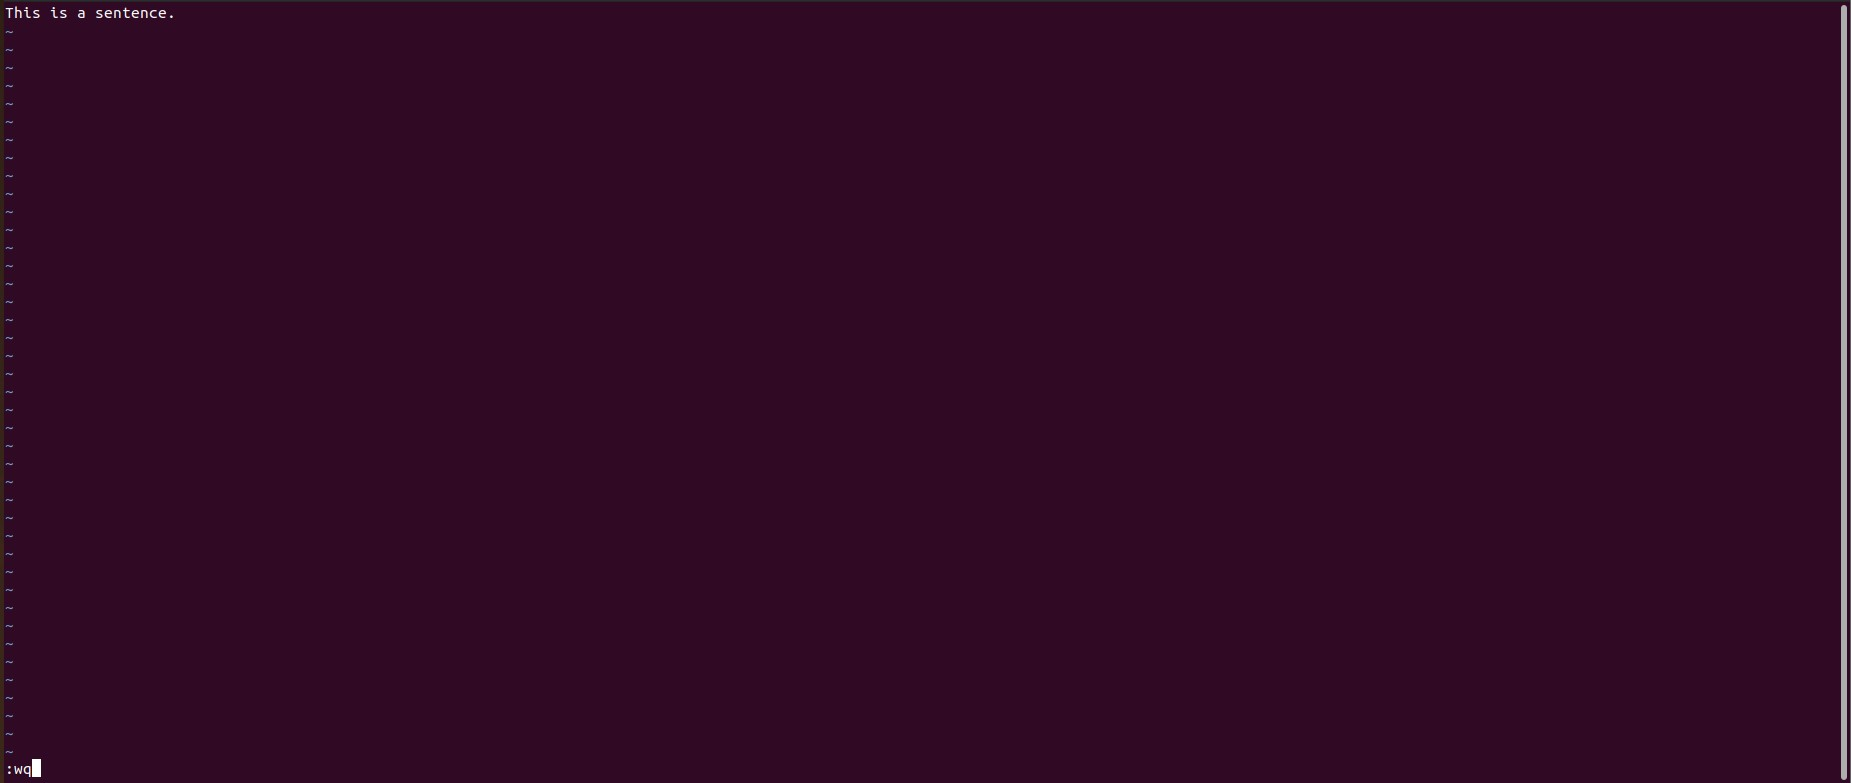
\includegraphics[width=1\textwidth]{021.jpg}
		
\includegraphics[width=1\textwidth]{022.jpg}
	\end{figure}
	
	\paragraph{(5)vim:}
	输入:help :w 打开 :w 命令的帮助文档	
	
	\begin{figure}[H]
		\centering
		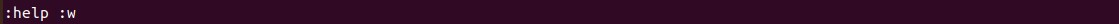
\includegraphics[width=1\textwidth]{023.jpg}
		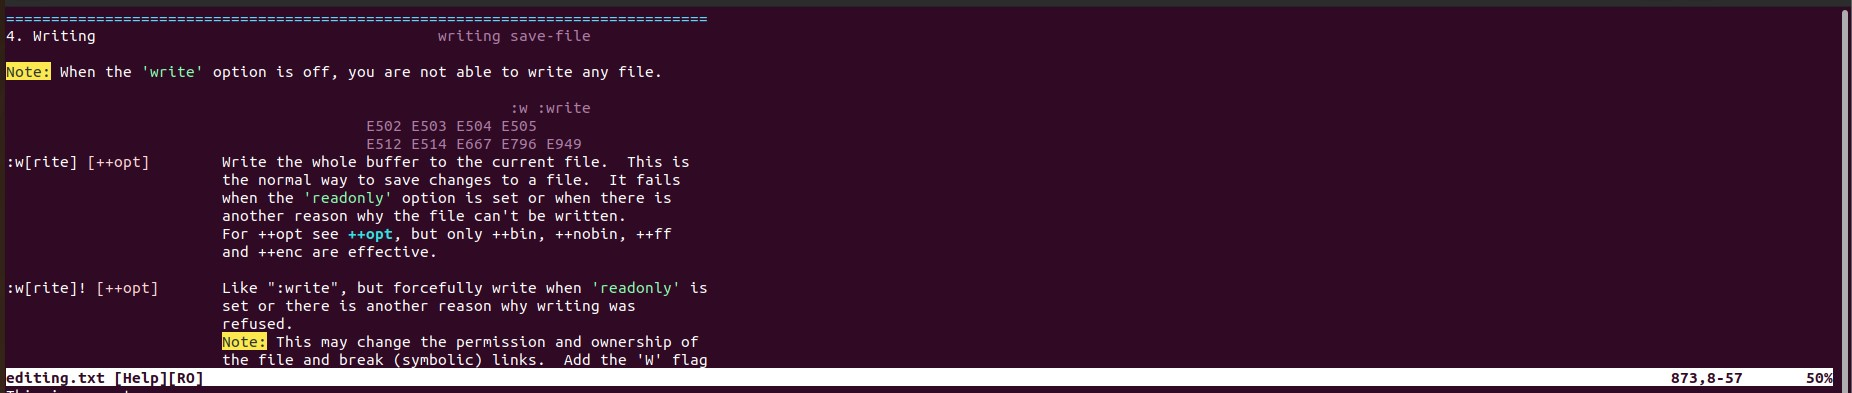
\includegraphics[width=1\textwidth]{024.jpg}
	\end{figure}
	
	\paragraph{(6)vim:}	
	输入:e {文件名} 打开要编辑的文件
	
	\begin{figure}[H]
		\centering
		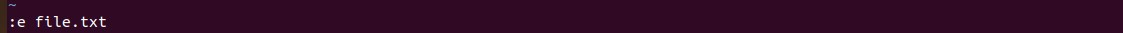
\includegraphics[width=1\textwidth]{025.jpg}
		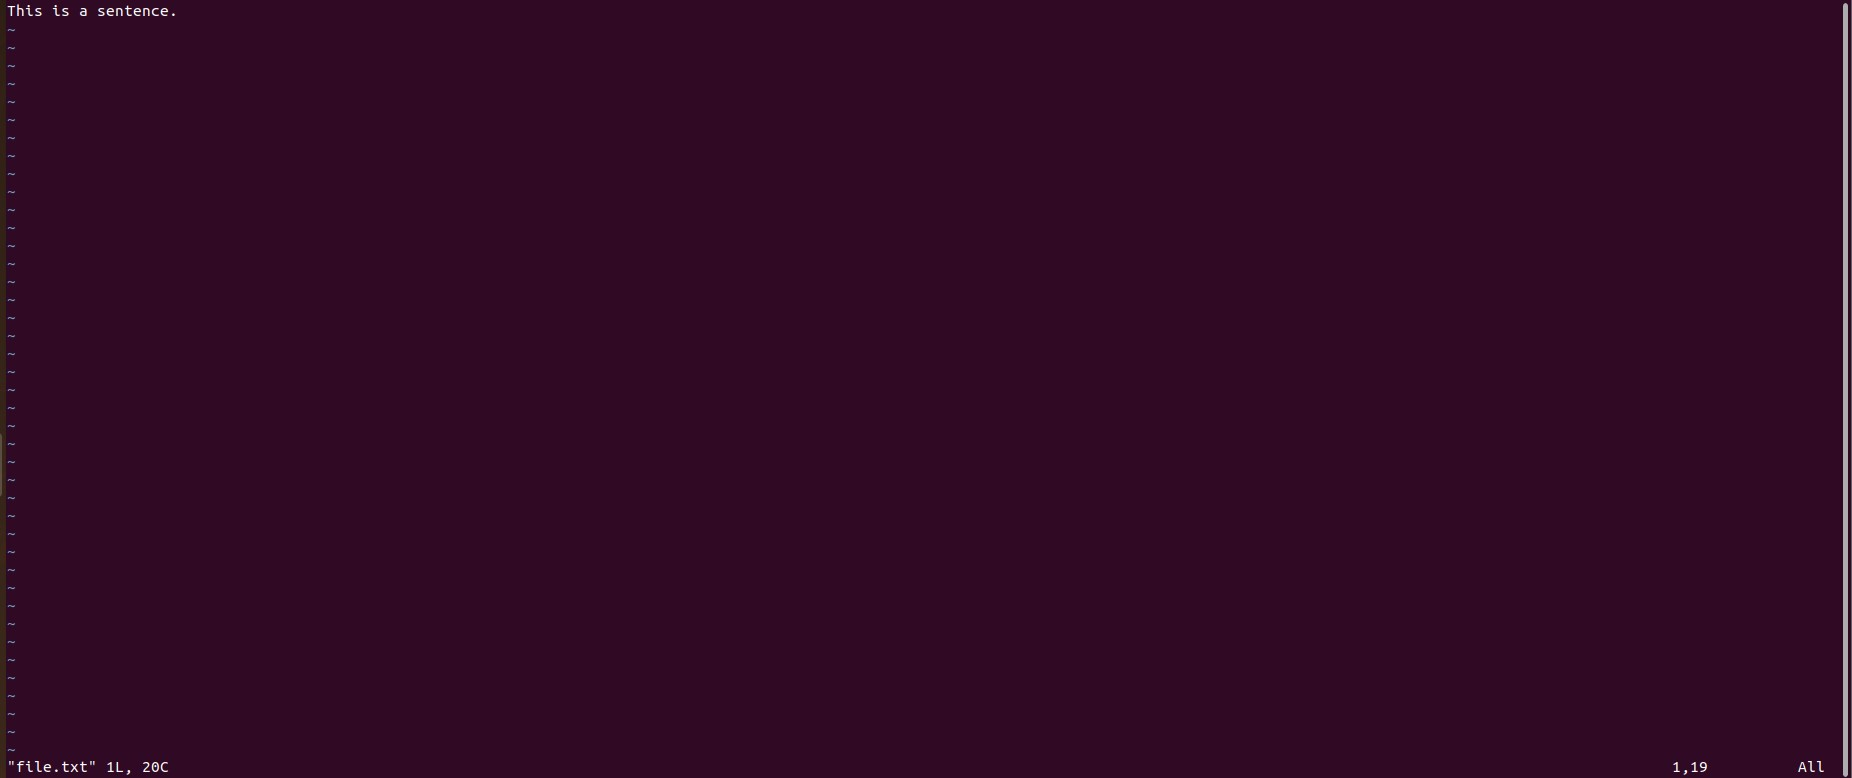
\includegraphics[width=1\textwidth]{026.jpg}
	\end{figure}
	
	\paragraph{(7)vim:}
	输入:ls 显示打开的缓存
	
	\begin{figure}[H]
		\centering
		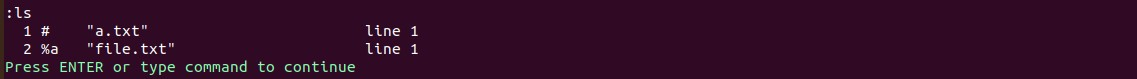
\includegraphics[width=1\textwidth]{027.jpg}
	\end{figure}
	
	\paragraph{(8)vim:}	
	打开一个文件,移动光标,在第二行行头和倒数第二行行尾插入文字。
	
	移动方式:
	
	基本移动: hjkl (左, 下, 上, 右)
	
	词: w (下一个词), b (词初), e (词尾)
	
	行: 0 (行初), \^ (第一个非空格字符), \$ (行尾)
	
	屏幕: H (屏幕首行), M (屏幕中间), L (屏幕底部)
	
	翻页: Ctrl-u (上翻), Ctrl-d (下翻)
	
	文件: gg (文件头), G (文件尾)
	
	行数: :{行数}<CR> 或者 {行数}G ({行数}为行数)
	
	杂项: \% (找到配对,比如括号或者 /* */ 之类的注释对)
	
	查找: f{字符}, t{字符}, F{字符}, T{字符}
	
	查找/到 向前/向后 在本行的{字符}
	
	, / ; 用于导航匹配
	
	搜索: /{正则表达式}, n / N 用于导航匹配
	
	\begin{figure}[H]
		\centering
		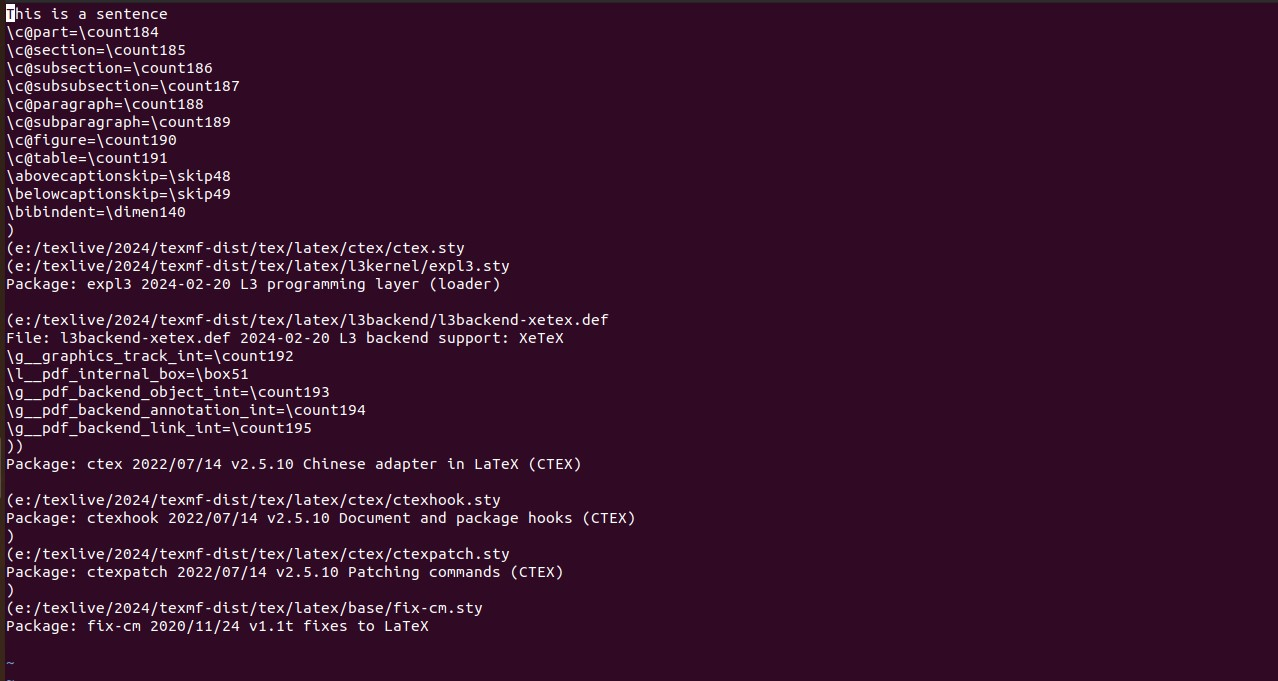
\includegraphics[width=1\textwidth]{028.jpg}
		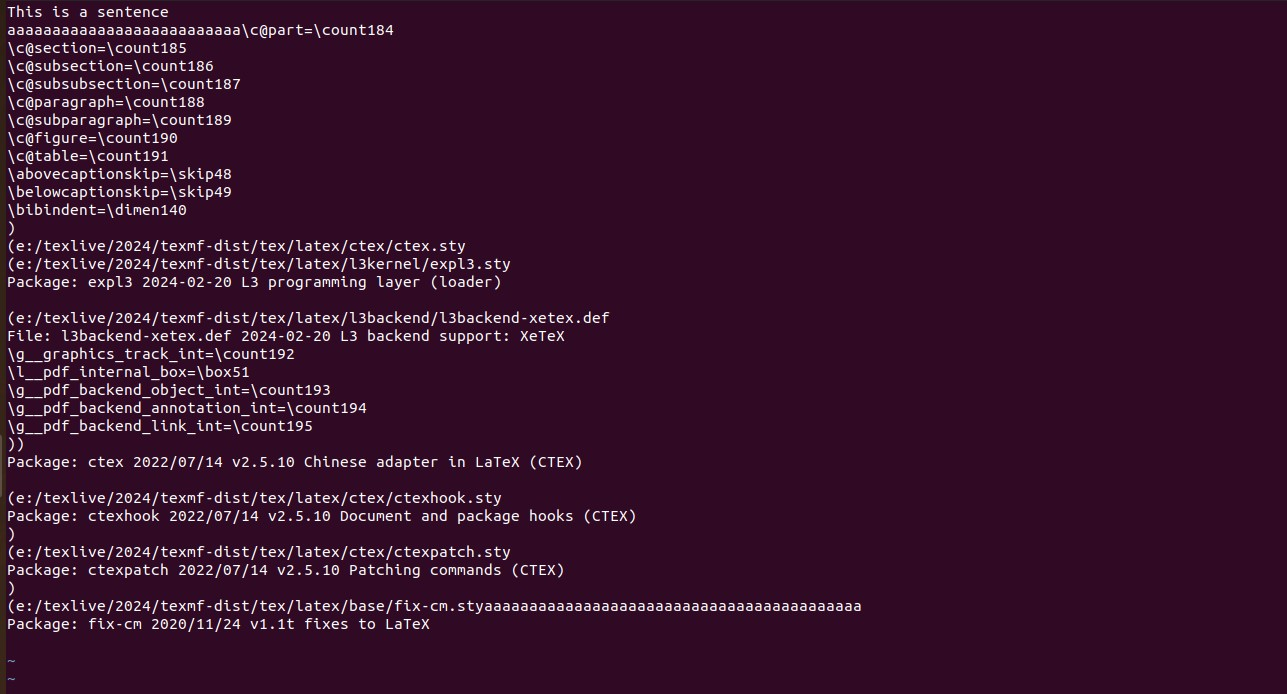
\includegraphics[width=1\textwidth]{029.jpg}
	\end{figure}
	
	\paragraph{(9)vim:}
	进入可视化模式选择部分内容。
	
	可视化:v
	
	可视化行: V
	
	可视化块:Ctrl+v	
	
	可以用移动命令来选中。
	
	\begin{figure}[H]
		\centering
		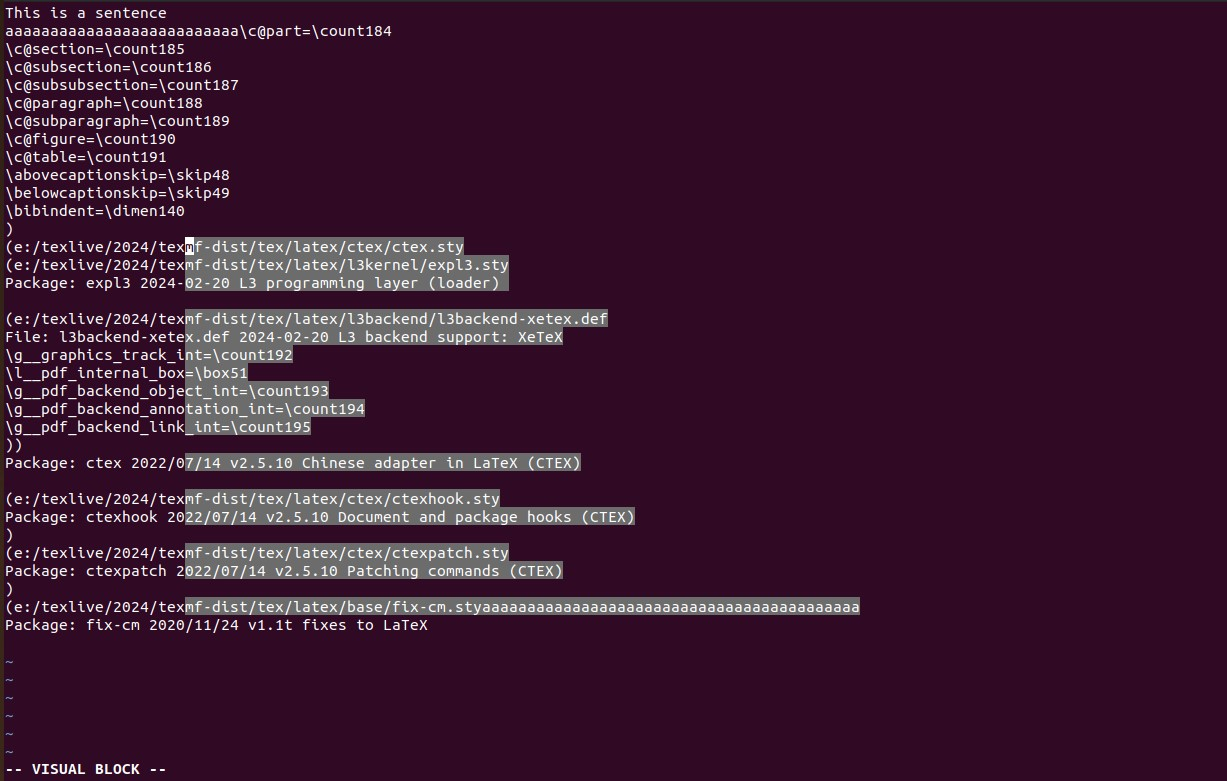
\includegraphics[width=1\textwidth]{030.jpg}
	\end{figure}
	
	\paragraph{(10)vim:}
	编辑文件,在最后一行行头删除7个词。(7dw)
	
	基本编辑操作:
	
	O / o 在之上/之下插入行
	
	d{移动命令} 删除 {移动命令}
	
	例如,dw 删除词, d\$ 删除到行尾, d0 删除到行头。
	
	c{移动命令} 改变 {移动命令}
	
	例如,cw 改变词
	
	比如 d{移动命令} 再 i
	
	x 删除字符(等同于 dl)
	
	s 替换字符(等同于 xi)
	
	可视化模式 + 操作
	
	选中文字, d 删除 或者 c 改变
	
	u 撤销, <C-r> 重做
	
	y 复制 / “yank” (其他一些命令比如 d 也会复制)
	
	p 粘贴
	
	~ 改变字符的大小写
	
	\begin{figure}[H]
		\centering
		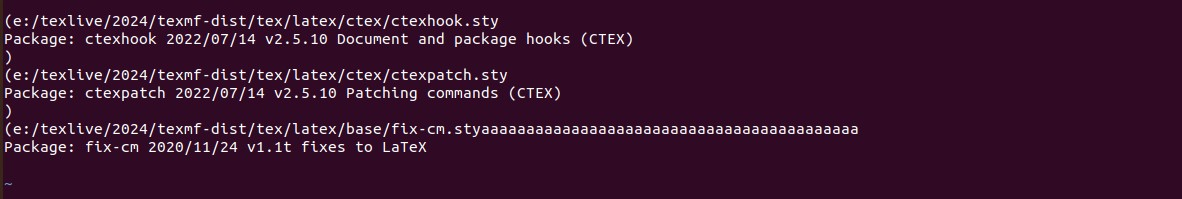
\includegraphics[width=1\textwidth]{031.jpg}
		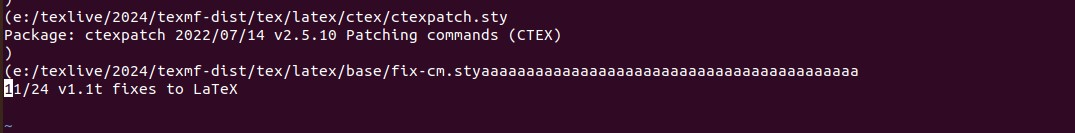
\includegraphics[width=1\textwidth]{032.jpg}
	\end{figure}
	
	\paragraph{(11)vim:}	
	修改以下实例fizz buzz,修复主函数没有被调用的问题。
	
	\begin{figure}[H]
	\centering
	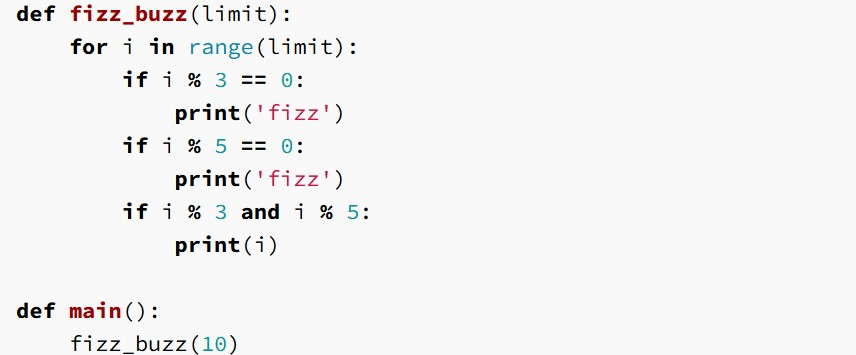
\includegraphics[width=1\textwidth]{033.jpg}
	\end{figure}

	答:-G 文件尾
	
	-o 向下打开一个新行
	
	-输入 “if name …”
	
	\begin{figure}[H]
		\centering
		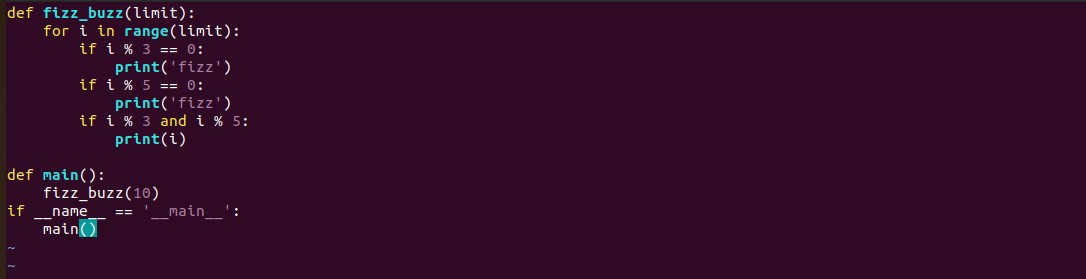
\includegraphics[width=1\textwidth]{034.jpg}
	\end{figure}
	
	\paragraph{(12)vim:}
	继续修改实例fizz buzz,修复从 0 而不是 1 开始的问题。
	
	答:-搜索 /range
	
	-ww 向后移动两个词
	
	-i 插入文字, “1, “
	
	-ea 在 limit 后插入, “+1”
	
	\begin{figure}[H]
		\centering
		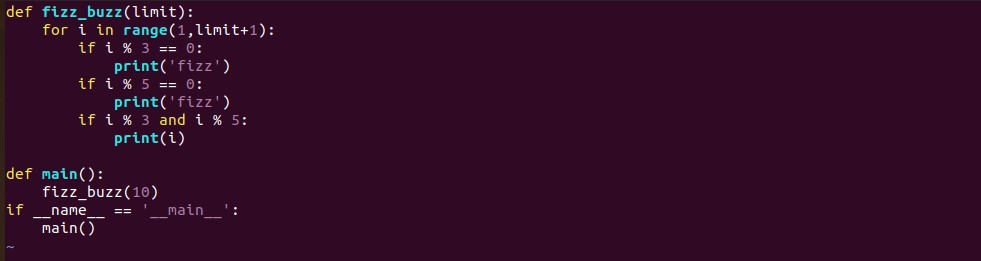
\includegraphics[width=1\textwidth]{035.jpg}
	\end{figure}
	
	\paragraph{(13)vim:}
	继续修改实例fizz buzz,在 5 的整数倍的时候打印 “buzz”。
	
	答:搜索/fizz,按n搜索下一个,一直到第三个"fizz“
	
	键入ci' ,再将“fizz”改为“buzz”
	
	\begin{figure}[H]
		\centering
		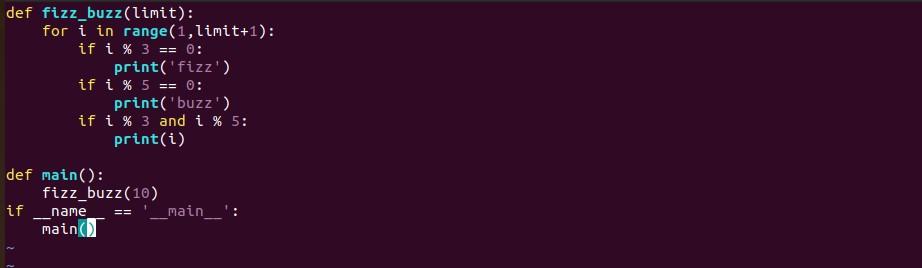
\includegraphics[width=1\textwidth]{036.jpg}
	\end{figure}
	
	\paragraph{(14)vim:}
	继续修改实例fizz buzz,在 15 的整数倍的时候在不同行打印 “fizz” 和 “buzz”。
	
	答:-jj\$i 插入文字到行尾
	
	-加入 “, end=’’”
	
	-jj. 重复第二个打印
	
	\begin{figure}[H]
		\centering
		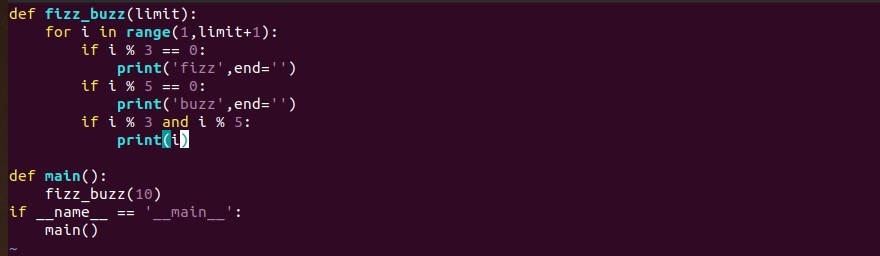
\includegraphics[width=1\textwidth]{037.jpg}
	\end{figure}
	
	\paragraph{(15)vim:}
	继续修改实例fizz buzz,采用硬编码的参数 10 而不是从命令控制行读取参数。
	
	答:gg回到文件头,O 向上打开新行
	
	键入内容“import sys”,然后回到normal模式
	
	键入/10,跳到10文字处
	
	键入ci( 命令,添加内容: int(sys.argv[1])
	
	\begin{figure}[H]
		\centering
		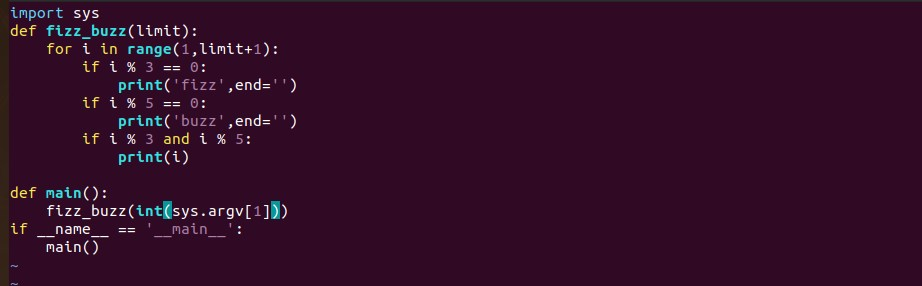
\includegraphics[width=1\textwidth]{038.jpg}
	\end{figure}
	
	\paragraph{(16)vim:}
	自定义 Vim。
	
	Vim 有一个位于 ~/.vimrc 的文本配置文件(包含 Vim 脚本命令)。
	
	我们提供一个文档详细的基本设置。下载我们提供的 vimrc,然后把它保存到 ~/.vimrc。 通读这个注释详细的文件 (用 Vim!), 然后观察 Vim 在这个新的设置下看起来和使用起来有哪些细微的区别。
	
	答:通读注释并实践可得该设置与默认设置的区别有以下几点:
	
	(1)语法高亮:会根据文件的类型自动进行语法高亮。
	
	(2)禁用默认启动消息:启动 Vim 时,不再显示默认的启动消息。
	
	(3)显示行号:每一行的左侧都会显示该行的行号,这有助于快速定位到代码中的特定位置。
	
	(4)相对行号:当同时启用 number 和 relativenumber 时,当前行的行号显示绝对行号,而其他行则显示相对于当前行的偏移量。
	
	(5)始终显示状态行:即使只打开一个窗口,Vim 也会在底部显示状态行。
	
	(6)Backspace 键行为改进:可以在任何位置使用 Backspace 键进行回退,包括插入点之前的位置。
	
	(7)允许隐藏未保存的缓冲区:通过 set hidden,可以隐藏包含未保存更改的缓冲区,而不会收到警告。
	
	(8)智能的搜索大小写敏感性:当搜索字符串全为小写时,搜索是大小写不敏感的;但如果搜索字符串包含大写字母,则搜索变为大小写敏感。
	
	(9)即时搜索:启用 incsearch 后,Vim 会随着您键入搜索字符串而即时显示搜索结果,而无需按 Enter 键。
	
	(10)重新映射方向键:通过 nnoremap 和 inoremap 命令,Vim 被配置为在尝试使用方向键时显示消息,鼓励用户使用更高效的移动命令。
	
	(11)禁用声音提示:noerrorbells 和 visualbell 的设置确保在出现错误时 Vim 不会发出声音,而是通过屏幕上的视觉提示来通知用户。
	
	(12)启用鼠标支持:set mouse+=a 允许用户在需要时使用鼠标进行选择和滚动。
	
	\begin{figure}[H]
		\centering
		
\includegraphics[width=1\textwidth]{041.jpg}
		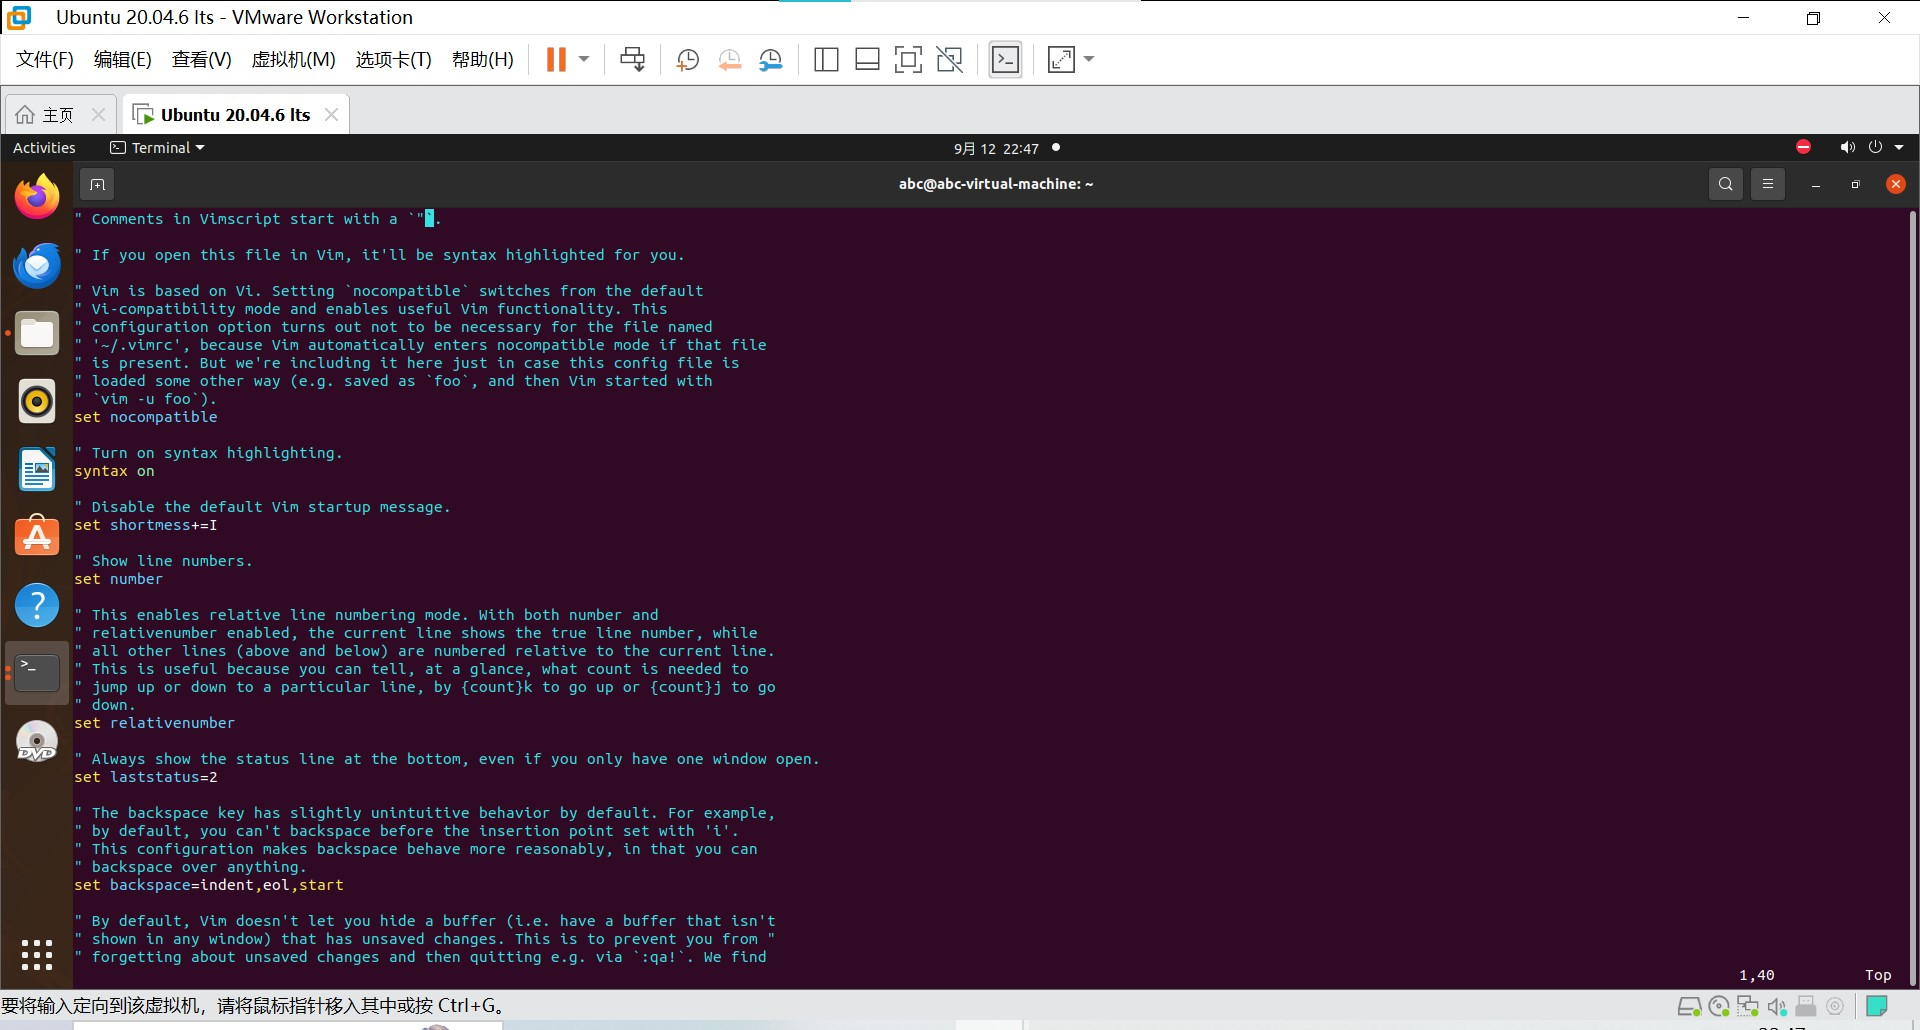
\includegraphics[width=1\textwidth]{039.jpg}
		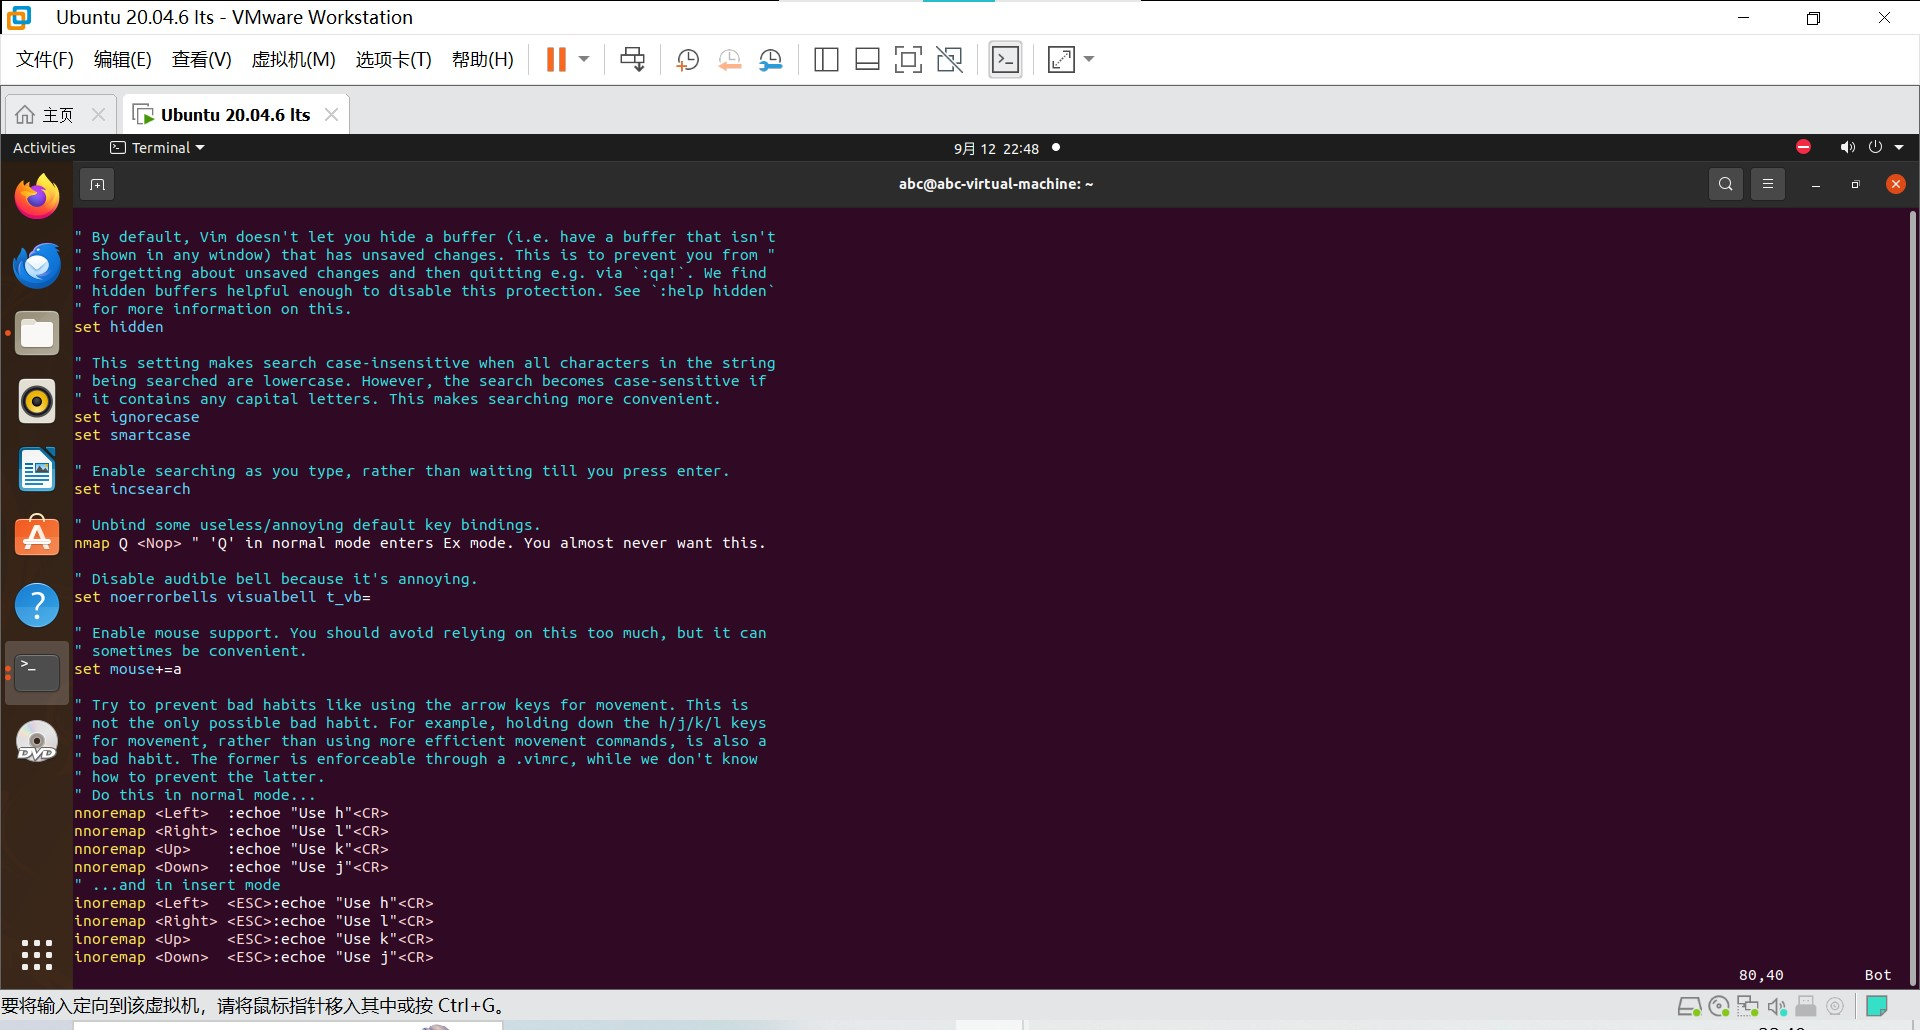
\includegraphics[width=1\textwidth]{040.jpg}
	\end{figure}
	
	\paragraph{(17)数据整理:}
	统计 words 文件 (/usr/share/dict/words) 中包含至少三个 a 且不以 's 结尾的单词个数。
	
	答:输入cat /usr/share/dict/words | tr "[:upper:]" "[:lower:]" | grep -E "\^([\^a]*a){3}.*\$" | grep -v "'s\$" | wc -l统计 words 文件中包含至少三个 a 且不以 's 结尾的单词个数,847个。
	
	\begin{figure}[H]
		\centering
		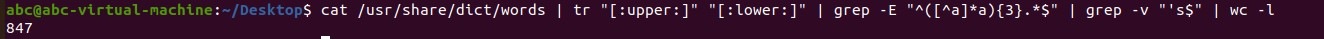
\includegraphics[width=1\textwidth]{042.jpg}
	\end{figure}
	
	\paragraph{(18)数据整理:}	
	这些单词中,出现频率前三的末尾两个字母是什么? sed 的 y 命令,或者 tr 程序也许可以帮你解决大小写的问题。
	
	答:输入cat /usr/share/dict/words | tr "[:upper:]" "[:lower:]" | grep -E "\^([\^a]*a){3}.*\$" | grep -v "'s\$" | sed -E "s/.*([a-z]{2})\$/$\backslash$1/" | sort | uniq -c | sort | tail -n3,结果如图。
	
	\begin{figure}[H]
		\centering
		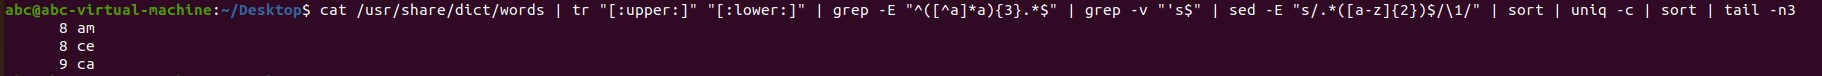
\includegraphics[width=1\textwidth]{043.jpg}
	\end{figure}
	
	\paragraph{(19)数据整理:}
	共存在多少种词尾两字母组合?
	
	答:输入cat /usr/share/dict/words | tr "[:upper:]" "[:lower:]" | grep -E "\^([\^a]*a){3}.*\$" | grep -v "'s\$" | sed -E "s/.*([a-z]{2})\$/$\backslash$1/" | sort | uniq | wc -l,共111种。
	
	\begin{figure}[H]
		\centering
		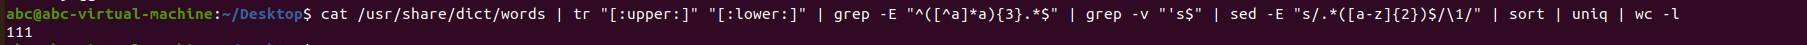
\includegraphics[width=1\textwidth]{044.jpg}
	\end{figure}
	
	\paragraph{(20)数据整理:}
	多少种组合从未出现过? (首先我们要生成一个包含全部组合的列表,然后再使用上面得到的出现的组合,比较二者不同即可。)
	
	答:写脚本生成包含全部组合的列表,再输入cat /usr/share/dict/words | tr "[:upper:]" "[:lower:]" | grep -E "\^([\^a]*a){3}.*\$" | grep -v "'s\$" | sed -E "s/.*([a-z]{2})\$/$\backslash$1/" | sort | uniq > occurance.txt得到出现的组合,然后比较两者不同diff --unchanged-group-format='' <(cat occurance.txt) <(cat all.txt) | wc -l,结果共565种。脚本已上传至github。
	
	\begin{figure}[H]
		\centering
		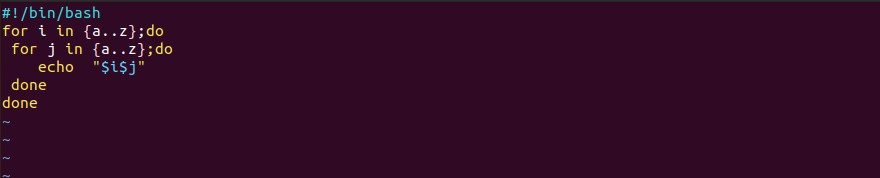
\includegraphics[width=1\textwidth]{045.jpg}
		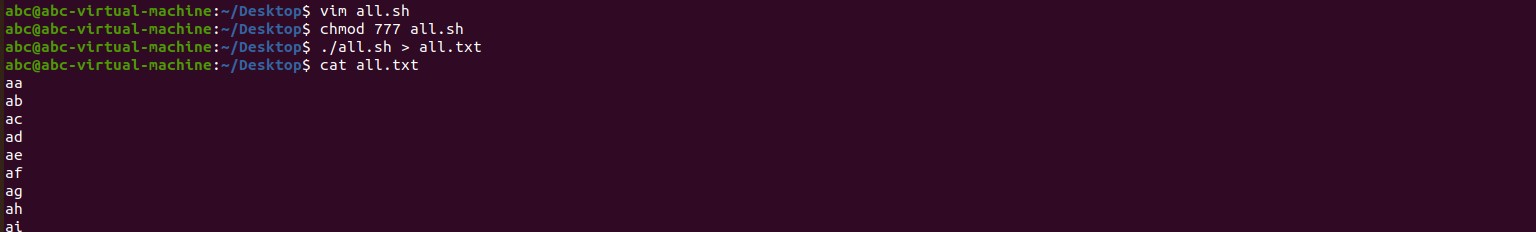
\includegraphics[width=1\textwidth]{046.jpg}
		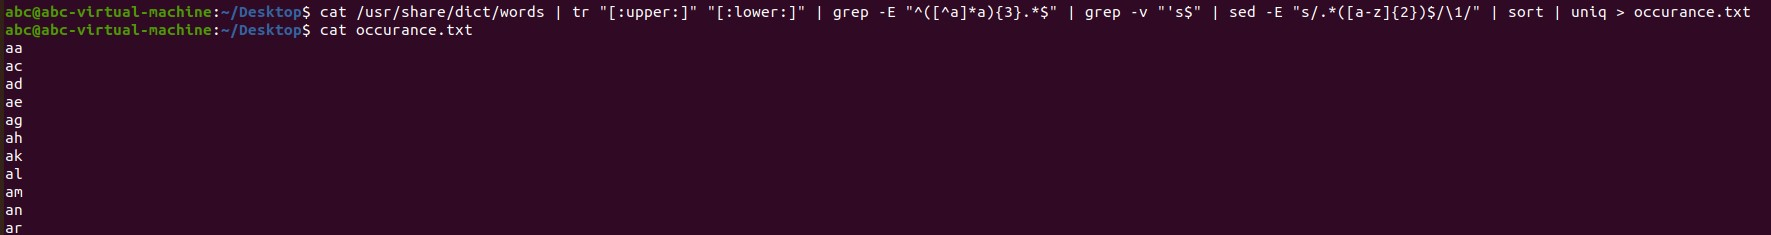
\includegraphics[width=1\textwidth]{047.jpg}
		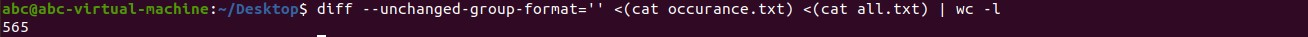
\includegraphics[width=1\textwidth]{048.jpg}
	\end{figure}
	
	\section{问题及解决方案}
	
	\paragraph{(1)}
	问题:在运行脚本时报错,如下图。
	
	\begin{figure}[h]
		\centering
		
\includegraphics[width=1\textwidth]{013.jpg}
	\end{figure}
	
	解决方案:修改脚本文件权限(chmod命令),再运行脚本。
	
	\begin{figure}[h]
		\centering
		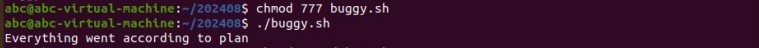
\includegraphics[width=1\textwidth]{014.jpg}
	\end{figure}
	
	\section{解题感悟}
	本实验中,我深入学习了Shell工具、Vim编辑器以及数据整理的相关操作,不仅巩固了理论知识,还通过实践提升了技能。
		
	在Shell工具方面,我通过练习题目,加深了对Shell命令的理解,并提升了编写脚本的能力,这对我在复杂环境中调试很有帮助。编写一个能够自动记录错误输出的bash脚本也让我认识到了脚本在自动化和错误追踪中的重要性。
	
	Vim编辑器的使用让我体验到了vim文本编辑器的强大与灵活。Vim的每一个命令都体现了其设计的精妙。
	
	数据整理部分的实验让我对文本处理工具有了更深入的了解。我学习了如何使用正则表达式和文本处理工具的组合来精确匹配和过滤数据,锻炼了我的数据处理能力。
	
	\section{github链接}
	\underline{https://github.com/zxm2580/xtkfgjjc-202408.git}	
	
\end{document}